% Signed subset sums of a Conway--Guy set, n=14 (generated by a script).
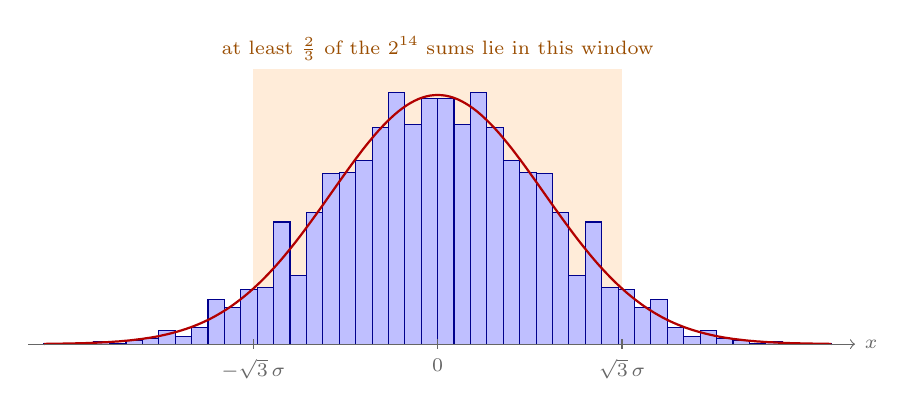
\begin{tikzpicture}[x=1cm,y=1cm]
\fill[orange!15] (-2.341,0) rectangle (2.341,3.5);
\draw[blue!55!black,fill=blue!25] (-5.000,0) rectangle (-4.792,0.003);
\draw[blue!55!black,fill=blue!25] (-4.792,0) rectangle (-4.583,0.003);
\draw[blue!55!black,fill=blue!25] (-4.583,0) rectangle (-4.375,0.003);
\draw[blue!55!black,fill=blue!25] (-4.375,0) rectangle (-4.167,0.038);
\draw[blue!55!black,fill=blue!25] (-4.167,0) rectangle (-3.958,0.003);
\draw[blue!55!black,fill=blue!25] (-3.958,0) rectangle (-3.750,0.041);
\draw[blue!55!black,fill=blue!25] (-3.750,0) rectangle (-3.542,0.069);
\draw[blue!55!black,fill=blue!25] (-3.542,0) rectangle (-3.333,0.176);
\draw[blue!55!black,fill=blue!25] (-3.333,0) rectangle (-3.125,0.100);
\draw[blue!55!black,fill=blue!25] (-3.125,0) rectangle (-2.917,0.214);
\draw[blue!55!black,fill=blue!25] (-2.917,0) rectangle (-2.708,0.568);
\draw[blue!55!black,fill=blue!25] (-2.708,0) rectangle (-2.500,0.465);
\draw[blue!55!black,fill=blue!25] (-2.500,0) rectangle (-2.292,0.694);
\draw[blue!55!black,fill=blue!25] (-2.292,0) rectangle (-2.083,0.725);
\draw[blue!55!black,fill=blue!25] (-2.083,0) rectangle (-1.875,1.551);
\draw[blue!55!black,fill=blue!25] (-1.875,0) rectangle (-1.667,0.867);
\draw[blue!55!black,fill=blue!25] (-1.667,0) rectangle (-1.458,1.668);
\draw[blue!55!black,fill=blue!25] (-1.458,0) rectangle (-1.250,2.167);
\draw[blue!55!black,fill=blue!25] (-1.250,0) rectangle (-1.042,2.183);
\draw[blue!55!black,fill=blue!25] (-1.042,0) rectangle (-0.833,2.336);
\draw[blue!55!black,fill=blue!25] (-0.833,0) rectangle (-0.625,2.748);
\draw[blue!55!black,fill=blue!25] (-0.625,0) rectangle (-0.417,3.200);
\draw[blue!55!black,fill=blue!25] (-0.417,0) rectangle (-0.208,2.789);
\draw[blue!55!black,fill=blue!25] (-0.208,0) rectangle (0.000,3.115);
\draw[blue!55!black,fill=blue!25] (0.000,0) rectangle (0.208,3.115);
\draw[blue!55!black,fill=blue!25] (0.208,0) rectangle (0.417,2.789);
\draw[blue!55!black,fill=blue!25] (0.417,0) rectangle (0.625,3.200);
\draw[blue!55!black,fill=blue!25] (0.625,0) rectangle (0.833,2.748);
\draw[blue!55!black,fill=blue!25] (0.833,0) rectangle (1.042,2.336);
\draw[blue!55!black,fill=blue!25] (1.042,0) rectangle (1.250,2.183);
\draw[blue!55!black,fill=blue!25] (1.250,0) rectangle (1.458,2.167);
\draw[blue!55!black,fill=blue!25] (1.458,0) rectangle (1.667,1.668);
\draw[blue!55!black,fill=blue!25] (1.667,0) rectangle (1.875,0.867);
\draw[blue!55!black,fill=blue!25] (1.875,0) rectangle (2.083,1.551);
\draw[blue!55!black,fill=blue!25] (2.083,0) rectangle (2.292,0.725);
\draw[blue!55!black,fill=blue!25] (2.292,0) rectangle (2.500,0.694);
\draw[blue!55!black,fill=blue!25] (2.500,0) rectangle (2.708,0.465);
\draw[blue!55!black,fill=blue!25] (2.708,0) rectangle (2.917,0.568);
\draw[blue!55!black,fill=blue!25] (2.917,0) rectangle (3.125,0.214);
\draw[blue!55!black,fill=blue!25] (3.125,0) rectangle (3.333,0.100);
\draw[blue!55!black,fill=blue!25] (3.333,0) rectangle (3.542,0.176);
\draw[blue!55!black,fill=blue!25] (3.542,0) rectangle (3.750,0.069);
\draw[blue!55!black,fill=blue!25] (3.750,0) rectangle (3.958,0.041);
\draw[blue!55!black,fill=blue!25] (3.958,0) rectangle (4.167,0.003);
\draw[blue!55!black,fill=blue!25] (4.167,0) rectangle (4.375,0.038);
\draw[blue!55!black,fill=blue!25] (4.375,0) rectangle (4.583,0.003);
\draw[blue!55!black,fill=blue!25] (4.583,0) rectangle (4.792,0.003);
\draw[blue!55!black,fill=blue!25] (4.792,0) rectangle (5.000,0.003);
\draw[red!70!black,line width=0.8pt] (-5.000,0.003)--(-4.950,0.004)--(-4.900,0.004)--(-4.850,0.005)--(-4.800,0.006)--(-4.750,0.007)--(-4.700,0.007)--(-4.650,0.009)--(-4.600,0.010)--(-4.550,0.011)--(-4.500,0.012)--(-4.450,0.014)--(-4.400,0.016)--(-4.350,0.018)--(-4.300,0.020)--(-4.250,0.023)--(-4.200,0.025)--(-4.150,0.028)--(-4.100,0.032)--(-4.050,0.035)--(-4.000,0.040)--(-3.950,0.044)--(-3.900,0.049)--(-3.850,0.055)--(-3.800,0.061)--(-3.750,0.067)--(-3.700,0.075)--(-3.650,0.082)--(-3.600,0.091)--(-3.550,0.100)--(-3.500,0.111)--(-3.450,0.122)--(-3.400,0.134)--(-3.350,0.147)--(-3.300,0.161)--(-3.250,0.176)--(-3.200,0.192)--(-3.150,0.209)--(-3.100,0.228)--(-3.050,0.248)--(-3.000,0.269)--(-2.950,0.292)--(-2.900,0.316)--(-2.850,0.342)--(-2.800,0.370)--(-2.750,0.399)--(-2.700,0.430)--(-2.650,0.463)--(-2.600,0.497)--(-2.550,0.534)--(-2.500,0.572)--(-2.450,0.612)--(-2.400,0.654)--(-2.350,0.698)--(-2.300,0.744)--(-2.250,0.791)--(-2.200,0.841)--(-2.150,0.893)--(-2.100,0.946)--(-2.050,1.001)--(-2.000,1.058)--(-1.950,1.117)--(-1.900,1.178)--(-1.850,1.240)--(-1.800,1.303)--(-1.750,1.368)--(-1.700,1.434)--(-1.650,1.502)--(-1.600,1.570)--(-1.550,1.639)--(-1.500,1.709)--(-1.450,1.779)--(-1.400,1.850)--(-1.350,1.921)--(-1.300,1.992)--(-1.250,2.063)--(-1.200,2.133)--(-1.150,2.203)--(-1.100,2.272)--(-1.050,2.340)--(-1.000,2.406)--(-0.950,2.472)--(-0.900,2.535)--(-0.850,2.596)--(-0.800,2.656)--(-0.750,2.713)--(-0.700,2.767)--(-0.650,2.819)--(-0.600,2.867)--(-0.550,2.913)--(-0.500,2.955)--(-0.450,2.994)--(-0.400,3.029)--(-0.350,3.060)--(-0.300,3.087)--(-0.250,3.111)--(-0.200,3.130)--(-0.150,3.145)--(-0.100,3.156)--(-0.050,3.162)--(0.000,3.164)--(0.050,3.162)--(0.100,3.156)--(0.150,3.145)--(0.200,3.130)--(0.250,3.111)--(0.300,3.087)--(0.350,3.060)--(0.400,3.029)--(0.450,2.994)--(0.500,2.955)--(0.550,2.913)--(0.600,2.867)--(0.650,2.819)--(0.700,2.767)--(0.750,2.713)--(0.800,2.656)--(0.850,2.596)--(0.900,2.535)--(0.950,2.472)--(1.000,2.406)--(1.050,2.340)--(1.100,2.272)--(1.150,2.203)--(1.200,2.133)--(1.250,2.063)--(1.300,1.992)--(1.350,1.921)--(1.400,1.850)--(1.450,1.779)--(1.500,1.709)--(1.550,1.639)--(1.600,1.570)--(1.650,1.502)--(1.700,1.434)--(1.750,1.368)--(1.800,1.303)--(1.850,1.240)--(1.900,1.178)--(1.950,1.117)--(2.000,1.058)--(2.050,1.001)--(2.100,0.946)--(2.150,0.893)--(2.200,0.841)--(2.250,0.791)--(2.300,0.744)--(2.350,0.698)--(2.400,0.654)--(2.450,0.612)--(2.500,0.572)--(2.550,0.534)--(2.600,0.497)--(2.650,0.463)--(2.700,0.430)--(2.750,0.399)--(2.800,0.370)--(2.850,0.342)--(2.900,0.316)--(2.950,0.292)--(3.000,0.269)--(3.050,0.248)--(3.100,0.228)--(3.150,0.209)--(3.200,0.192)--(3.250,0.176)--(3.300,0.161)--(3.350,0.147)--(3.400,0.134)--(3.450,0.122)--(3.500,0.111)--(3.550,0.100)--(3.600,0.091)--(3.650,0.082)--(3.700,0.075)--(3.750,0.067)--(3.800,0.061)--(3.850,0.055)--(3.900,0.049)--(3.950,0.044)--(4.000,0.040)--(4.050,0.035)--(4.100,0.032)--(4.150,0.028)--(4.200,0.025)--(4.250,0.023)--(4.300,0.020)--(4.350,0.018)--(4.400,0.016)--(4.450,0.014)--(4.500,0.012)--(4.550,0.011)--(4.600,0.010)--(4.650,0.009)--(4.700,0.007)--(4.750,0.007)--(4.800,0.006)--(4.850,0.005)--(4.900,0.004)--(4.950,0.004)--(5.000,0.003);
\draw[->,black!60] (-5.20,0)--(5.30,0) node[right,font=\scriptsize]{$x$};
\draw[black!60] (-2.341,0.06)--(-2.341,-0.06) node[below,font=\scriptsize]{$-\sqrt3\,\sigma$};
\draw[black!60] (2.341,0.06)--(2.341,-0.06) node[below,font=\scriptsize]{$\sqrt3\,\sigma$};
\draw[black!60] (0.000,0.06)--(0.000,-0.06) node[below,font=\scriptsize]{$0$};
\node[font=\scriptsize,align=center,orange!60!black] at (0,3.75) {at least $\frac23$ of the $2^{14}$ sums lie in this window};
\end{tikzpicture}
